\section{Presentation Interface}

The concept of this interface is to keep the user from accessing their devices, just to check the current playlist configuration, and instead provide quick and easily accessible overview for the users of the system. By having a separated screen from the users' devices, the system may reduce the amount of time users spend using these devices, which was declared a problem best seen minimized, concluded in \cref{sub:user_requirements}. The intention is to have the playlist on a screen above the bar, as visually envisioned in \cref{fig:PresentationInterface}. This should direct the users eyes towards the bar, if they are interested in viewing the current results, by making it more accessible to the user as the screen is bigger in size and always on, opposed to the small handheld device \cite{DEB} . It is important to stress that the screen should not be visually blockable by a person or other objects.

This is a part of the system which should always be visually accessible to the user, therefore should also be visually pleasing to look at, but still contain all the information needed by the user. An interesting problem to solve, is having to display each individual's votes in an efficient way, without providing an overflow of information, confusing the user. One suggested solution is to have the most distinguishing content to the left with the reading direction, and the least distinguishing content to the right \cite{material}. In this case, a tracks placement on the playlist to the left and the users who voted for it on the right. Depicting individual users will require some sort of id, through a login or similar, to distinguish users.

\begin{figure}[hbtp]
  \centering
  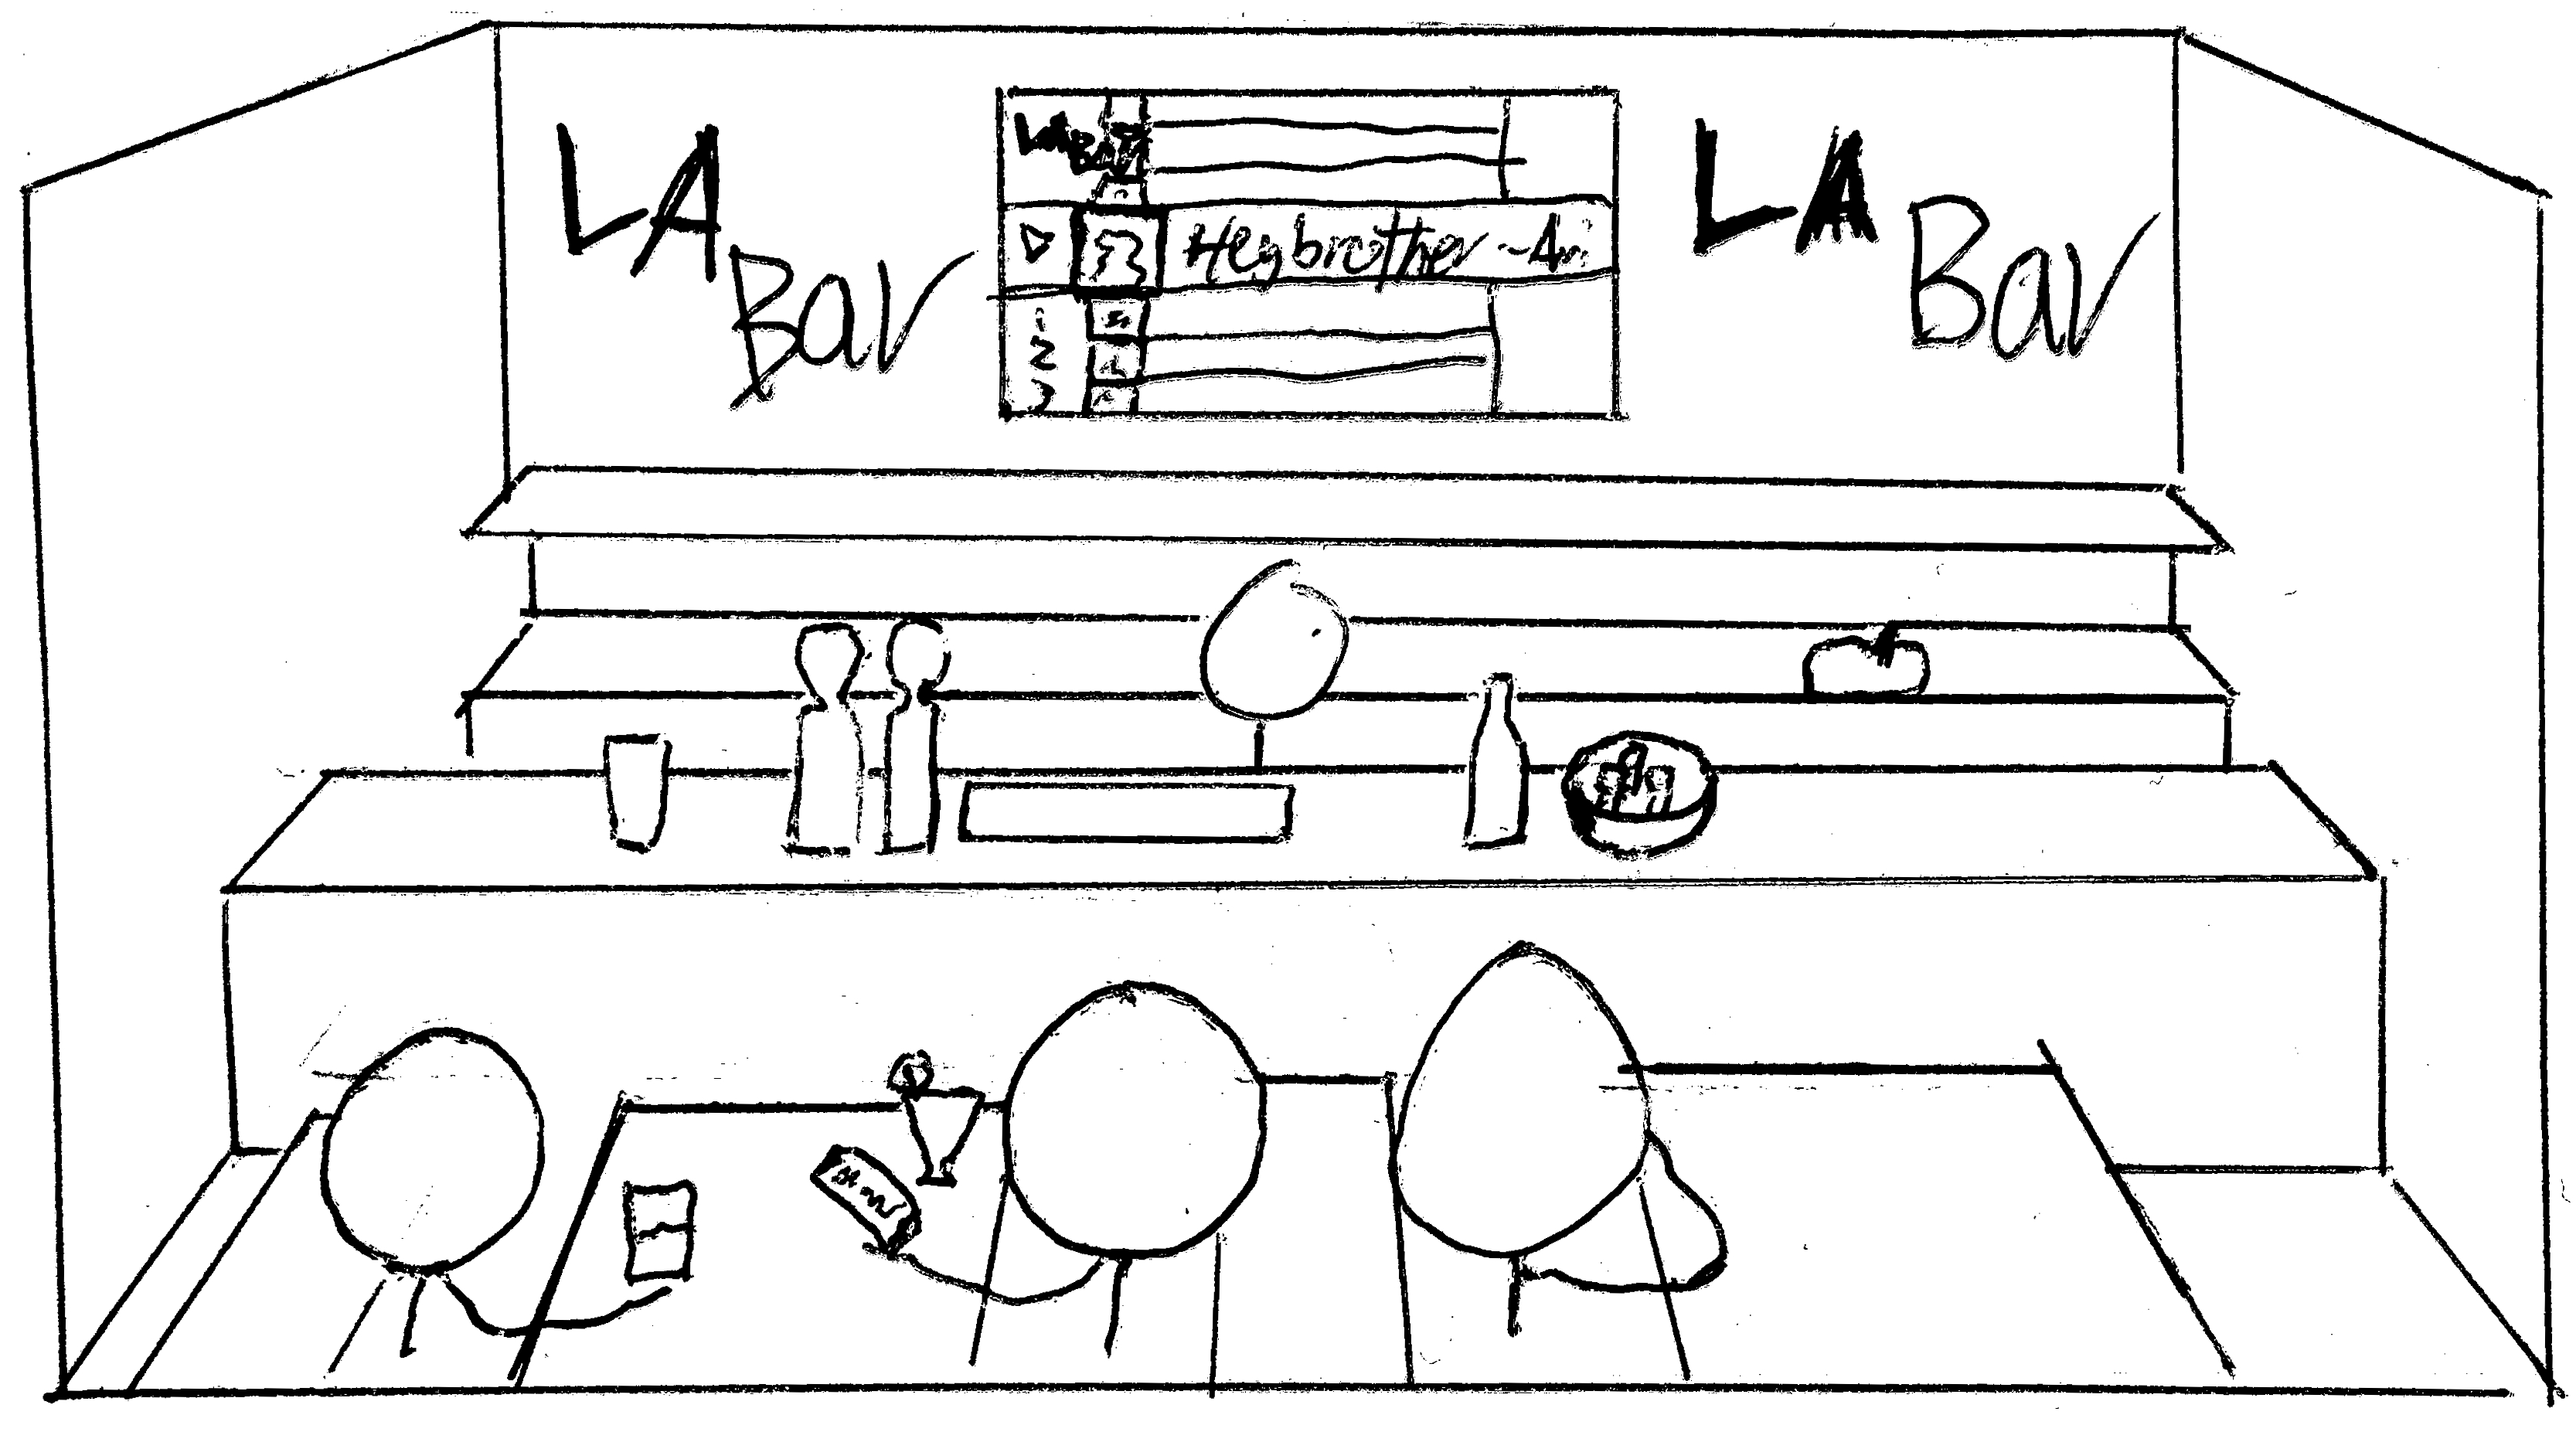
\includegraphics[width=1.0\linewidth]{Images/presentation.png}
  \caption{Sketch of the screen in context and visual design.}\label{fig:PresentationInterface}
\end{figure}

\begin{figure}[hbtp]
  \centering
  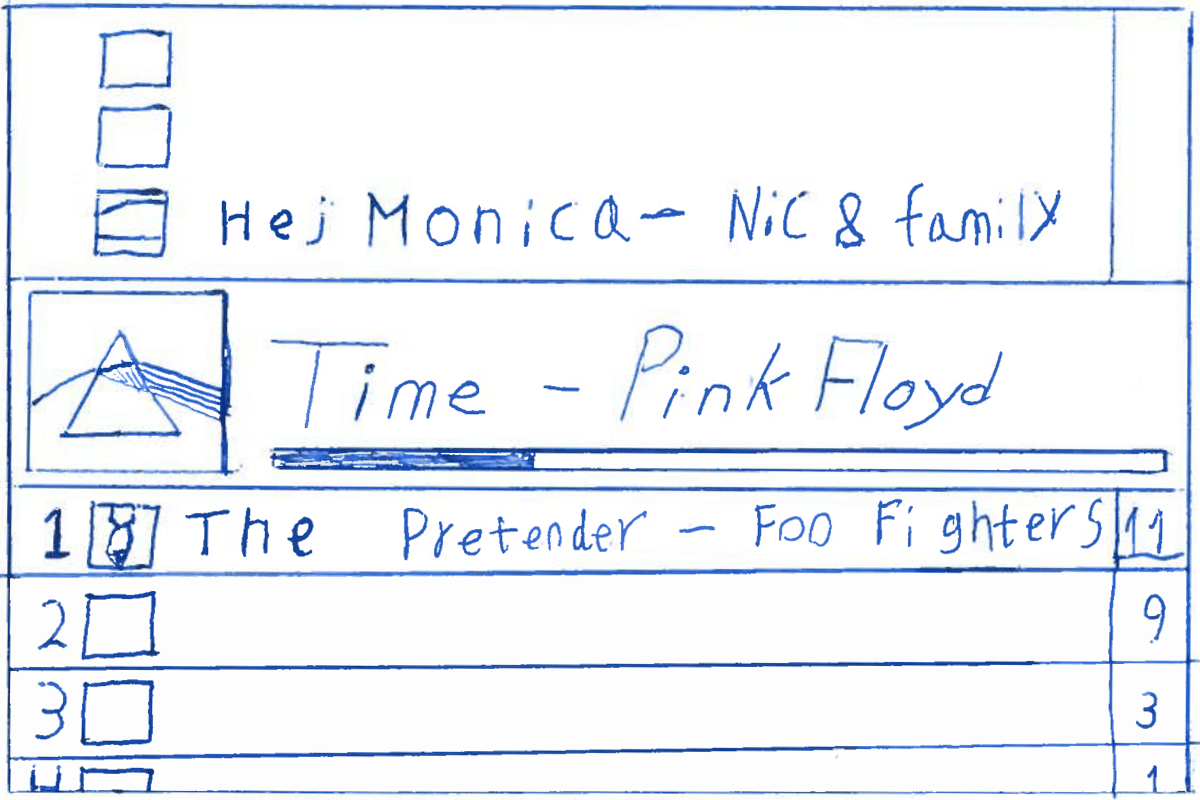
\includegraphics[width=1.0\linewidth]{Images/presentationInterface.png}
  \caption{A Sketch of the visual design of the presentation interface.}\label{fig:presentation}
\end{figure}

The presentation view is designed to show the current playing song, the history and the tracks to be played next, according to the current votes. The currently playing song will be shown in the vertical middle of the screen. The history will be displayed above as a list of tracks, ordered with the last played track at the button. Below the current playing track a list of tracks will display the songs people have voted on. The highest voted song will be in the top of the list as shown on figure \cref{fig:presentation}. 


\alnote{skriv mere}

%Sørensen and Kjeldskov did an article on interaction with a similar system. They found some field test 
